\section{Numerical test cases}
\label{sec:num_cases}
In this section we present solutions to the linear advection equation using the C1FR scheme to show that it is stable and achieves the theoretical order of convergence of $P+1$ when the solution is discretized with an order $P$ polynomial. In addition, we present solutions to the linear advection-diffusion equation to demonstrate the ability to change the scheme's dispersion and dissipation properties while maintaining stability. As a test of the scheme's ability to solve non-linear systems of equations, solutions to Sod's Shock Tube problem \cite{roe1981approximate} and Einfeldt et al.'s 123 Problem \cite{einfeldt1991godunov} are presented. The solution of these challenging, difficult to stabilize initial conditions of the Euler equations would be a testament to the CMFR's promise as a numerical scheme with built-in stability.

As can be seen from the derivation of the \gls{c1fr} scheme, the interface flux constants $\alpha_0$ and $\alpha_1$, the norm constants $c_0$ and $c_1$, and the location of the solution points at each element are variable. In this exposition, we will not modify the location of the solution points and use the standard zeroes of the Legendre polynomials. We note that the values of $c_1$ have a direct impact on the scheme's dispersion and dissipation, while --as expected-- the $\alpha_r$ values affect the dissipation only. A future rigorous Fourier analysis would reveal wiser choices for the $c_1$ parameter.

In the case of the Euler equations, the solution points in an element are located at the zeroes of the Legendre polynomials plus the end-points. It was found that the absence of solution points at, or very close to, the edges of an element would de-stabilize the scheme. This is to be expected, given that extrapolation of a polynomial is prone to large over and under-shoots of the real values.

\subsection{Order of Accuracy of C1FR}
\subsubsection{Setup}

The 1-D experiments follow the procedure suggested by Vincent et al.~\cite{vincent2011insights} to estimate  a scheme's order of accuracy isolating interpolation errors. We solve the linear advection equation with advection speed of $a = 1$. The domain was $\Omega = [-10, 10]$ and was discretized in $n = 10, 15, 24, 38, 60$ equispaced elements of orders $P = 1,2,3$. The initial condition was a sine wave with wavenumber $k = 2\pi/20 \approx 0.63$. The advection speed was $1$ and fully upwinded fluxes $\alpha_0 = 0, \alpha_1 = 0$ in Eqn. \eqref{eq:ifluxdef}) were used. The boundary conditions were periodic. The simulation advanced using a fourth order \gls{rk} scheme with a time-step of order $10^{-3}$.

The initial condition was advected for a full domain length, using either standard nodal DG or \gls{c1fr}, and the resulting solution was taken as the reference solution $u_{ref}$. The wave was advected for a further full domain length to obtain the final solution $u_{final}$. The error was calculated by taking the L-2 norm of $u_{ref} - u_{final}$.

\subsubsection{Results and discussion}
Figures \ref{fig:adv_P1},\ref{fig:adv_P2}, and \ref{fig:adv_P3} show the rate of convergence of the solution and its derivative obtained by discretizing the solution wih polynomials of order $P = 1,2,3$, respectively. The slopes of the best fit lines are presented in each figure's caption.

\begin{figure}[h]
\centering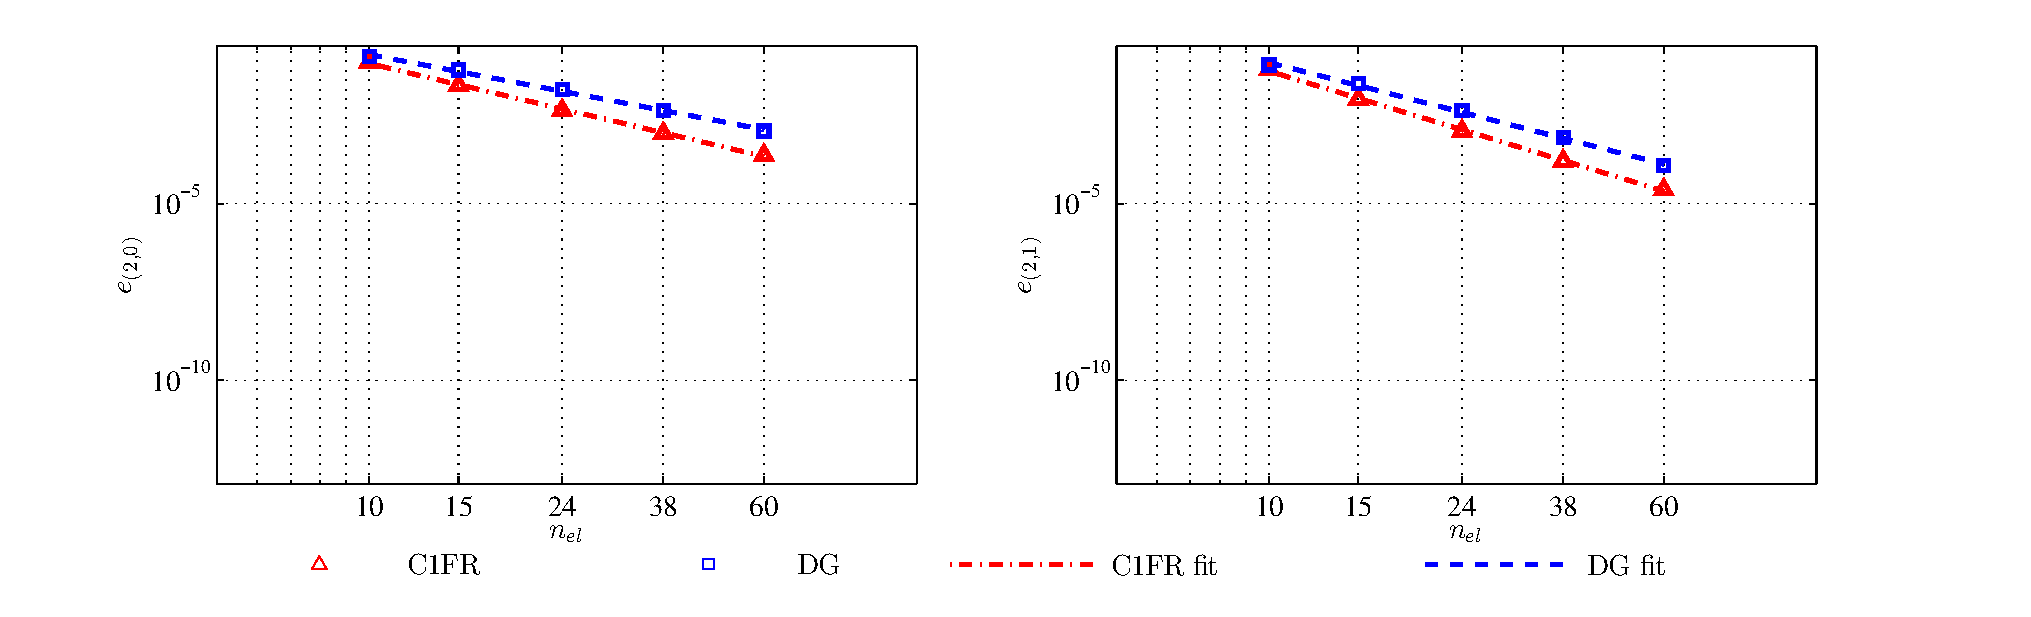
\includegraphics[width=1\textwidth,trim=\Ltrim cm 0cm \Rtrim cm 0cm]{\cmfrdir/Figures/Order_accuracy/P_1}
\caption{L-2 norm of error of advected sine wave and its derivative, $e_{(2,0)}$ and $e_{(2,1)}$ respectively, versus number of elements, for linear advection with polynomial discretization of order $P = 1$. Order of accuracy in solution: \gls{dg}: $2.728$, \gls{c1fr}: $3.374$. Order of accuracy in first derivative: \gls{dg}: $2.691$, \gls{c1fr}: $3.359$.}
\label{fig:adv_P1}
\end{figure}

\begin{figure}[h]
\centering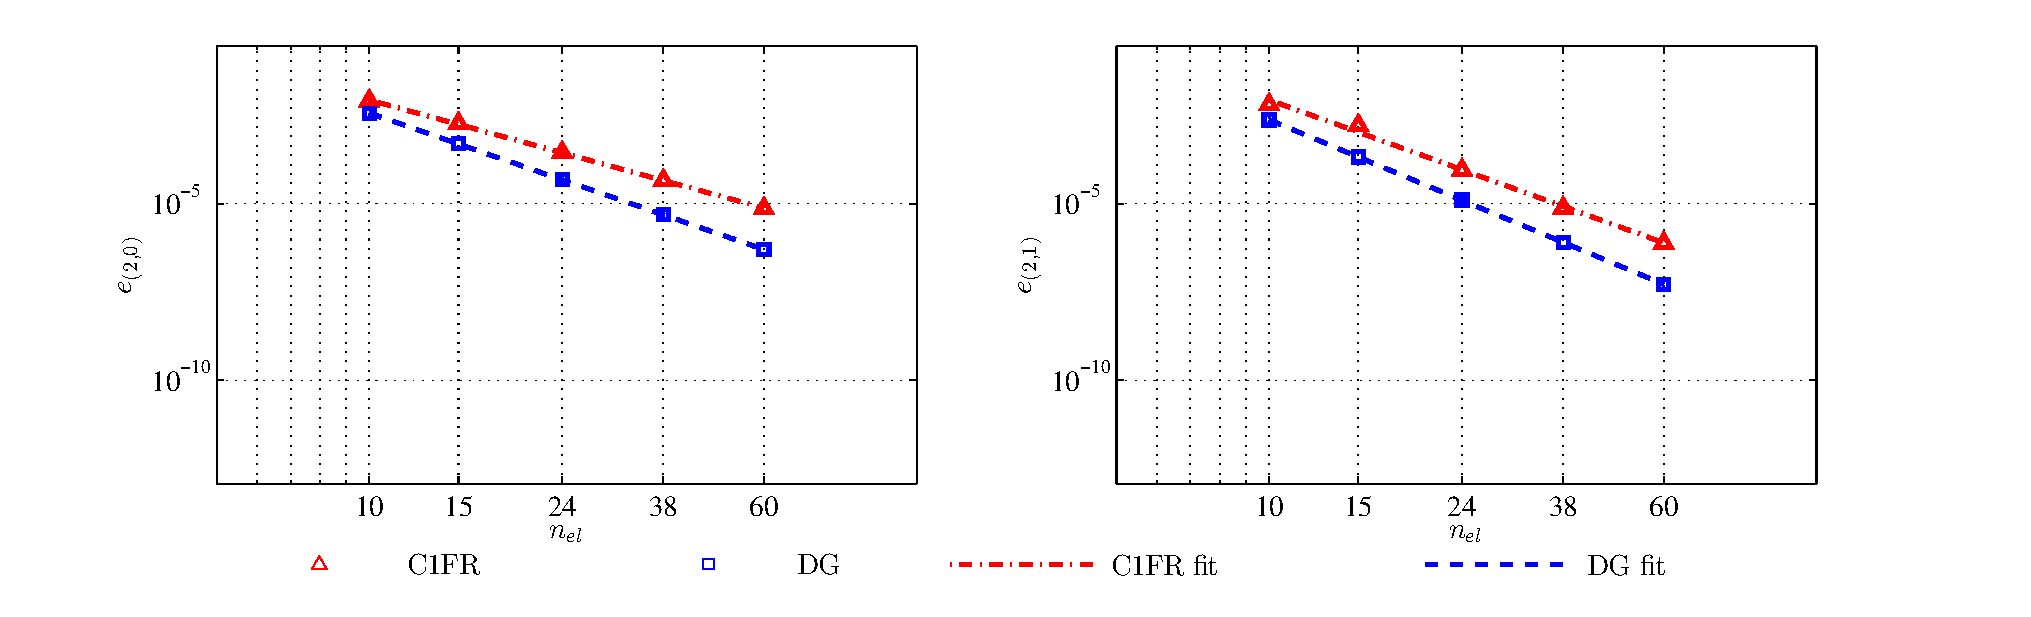
\includegraphics[width=1\textwidth,trim=\Ltrim cm 0cm \Rtrim cm 0cm]{\cmfrdir/Figures/Order_accuracy/P_2}
\caption{L-2 norm of error of advected sine wave and its derivative, $e_{(2,0)}$ and $e_{(2,1)}$ respectively, versus number of elements, for linear advection with polynomial discretization of order $P = 2$. Order of accuracy in solution: \gls{dg}: $4.960$, \gls{c1fr}:  $3.917$ . Order of accuracy in first derivative: \gls{dg}: $4.971$, \gls{c1fr}: $4.178$.}
\label{fig:adv_P2}
\end{figure}

\begin{figure}[h]
\centering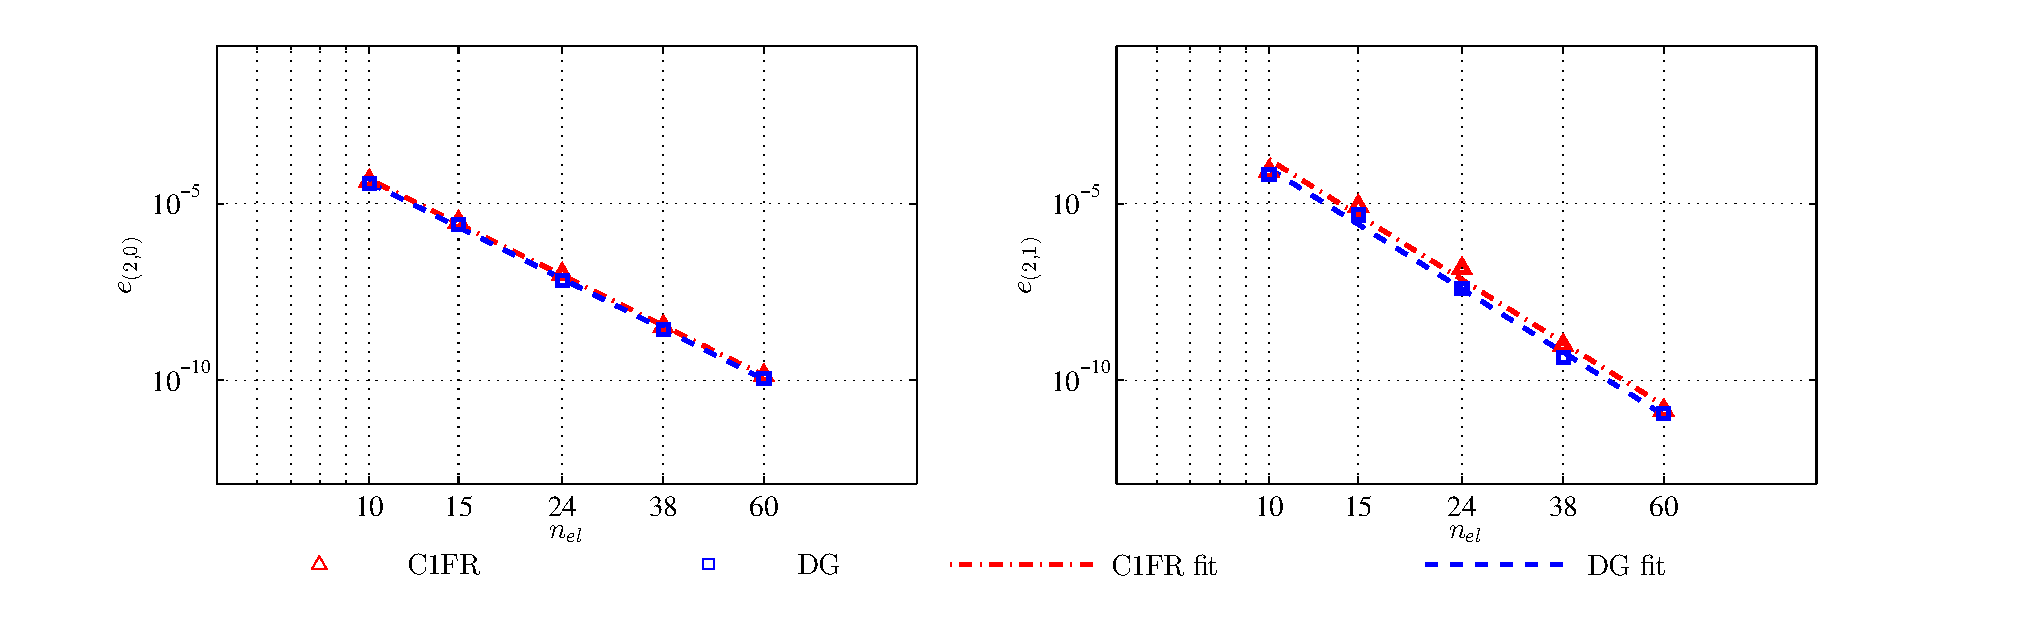
\includegraphics[width=1\textwidth,trim=\Ltrim cm 0cm \Rtrim cm 0cm]{\cmfrdir/Figures/Order_accuracy/P_3}
\caption{L-2 norm of error of advected sine wave and its derivative, $e_{(2,0)}$ and $e_{(2,1)}$ respectively, versus number of elements, for linear advection with polynomial discretization of order $P = 3$. Order of accuracy in solution: \gls{dg}: 7.119, \gls{c1fr}: 7.187. Order of accuracy in first derivative: \gls{dg}: 7.908, \gls{c1fr}: 7.882.}
\label{fig:adv_P3}
\end{figure}

The fact that we recover the expected nodal \gls{dg}'s $2P+1$ order of convergence found by Vincent et al. \cite{vincent2011insights} for $P = 1,2,3$ validates the experimental setup. It is interesting to note that \gls{c1fr} retains \gls{fr}'s even-odd order of convergence behavior: when $P$ is odd, the order of convergence is $2P+1$; while when $P$ is even, the order of convergence is $2P$.

This numerical experiment does not replace a von Neumann analysis, but does show that the scheme is stable, consistent, and maintains the desired order of accuracy. Although we would not expect the scheme to maintain super-convergence properties in real applications --as the interpolation errors are themselves of order $P+1$--, this experiment relieves worries about C1FR's introducing lower order errors.

\subsection{Advection-Diffusion Energy Preservation}
\label{sec:advDiff}
Motivated by the fact that in turbulent simulations the preservation of energy at different scales (or wavenumbers) is of paramount importance, we wanted to explore the potential benefit of having sets of families of stable numerical schemes with modifiable dispersion and dissipation properties.

By solving the linear advection-diffustion equation we are able to assess how much dissipation in different scales is due to numerics as opposed to the nature of the equation.

\subsubsection{Setup}

In these numerical experiments we solve the linear advection-diffusion equation using the C1FR and nodal DG schemes following the approach described by Huynh \cite{huynh2009reconstruction}. In essense, we re-write the diffusion-advection equation as a system of two first order \gls{pde}s as follows
\begin{equation}
\begin{split}
\dd{u}{t} + \dd{q}{x} = 0 \\
q - au + \kappa\dd{u}{x} = 0
\end{split}
\end{equation}

where $a$ is the advection speed, $\kappa$ is the diffusion coefficient, and $q$ is a dummy variable. The desired scheme is used to discretize the spatial differentiation.

In this section, we let $a = 1$, $\kappa = 10^{-2}$. The domain was $\Omega = [-10,10]$ and was discretized in $n = 20$ equispaced elements of polynomial order $P = 5$. The boundary conditions were periodic. The initial conditions were sine waves with low, medium, and high wavenumbers. The wavenumbers were chosen relative to the Nyquist limit of the discretization: 
\[k = \rho (P+1)\pi/h\]
 where $\rho$ is a non-dimensional constant, $P+1$ is the number of solution points in each element of polynomial degree $P$, and $h$ is the size of the element. Note that when $\rho = 1$, the Nyquist limit is reached exactly if the solution points are spaced evenly.

In our experiments, for the low wavenumber $\rho = 0.25$; medium wavenumber $\rho = 0.5$; high wavenumber $\rho = 0.75$. The fluxes were all fully upwinded and in the \gls{c1fr} scheme, $c_1 = -5\cdot10^{-3}$. The solution is advanced with a standard \gls{rk}4 time-stepping scheme. A \gls{cfl} of $0.3$ is used for both schemes. At each timestep, we calculate the square of the L-2 norm of the solution and its derivative, and compare it to the exact corresponding values. $||u||_{(2,m)} $ is the L-2 norm of the $m^{\text{th}}$ derivative of solution $u$.


\subsubsection{Results and discussion}
Fig. \ref{fig:low_wavenumber} shows that both schemes preserve the exact solution and derivative norms of the low wavenumber. On the other hand, \ref{fig:high_wavenumber} shows that both schemes suffer from aliasing and deviate significantly from the exact L-2 norms when the initial solution is a high wavenumber. \gls{c1fr} is somewhat closer to the exact values than nodal \gls{dg} both before and after the norms of the numerical solutions intersect the exact solution's L-2 norm.

Fig. \ref{fig:medium_wavenumber} presents a promising result. \gls{c1fr} preserves the correct L-2 norms of the solution while nodal \gls{dg}'s numerical dissipation affects the energy content of the wave. The L-2 norm of C1FR's solution derivative oscillates around the exact value, while nodal \gls{dg}'s oscillates with similar magnitude trending further below the exact values.


\begin{figure}[h]
\centering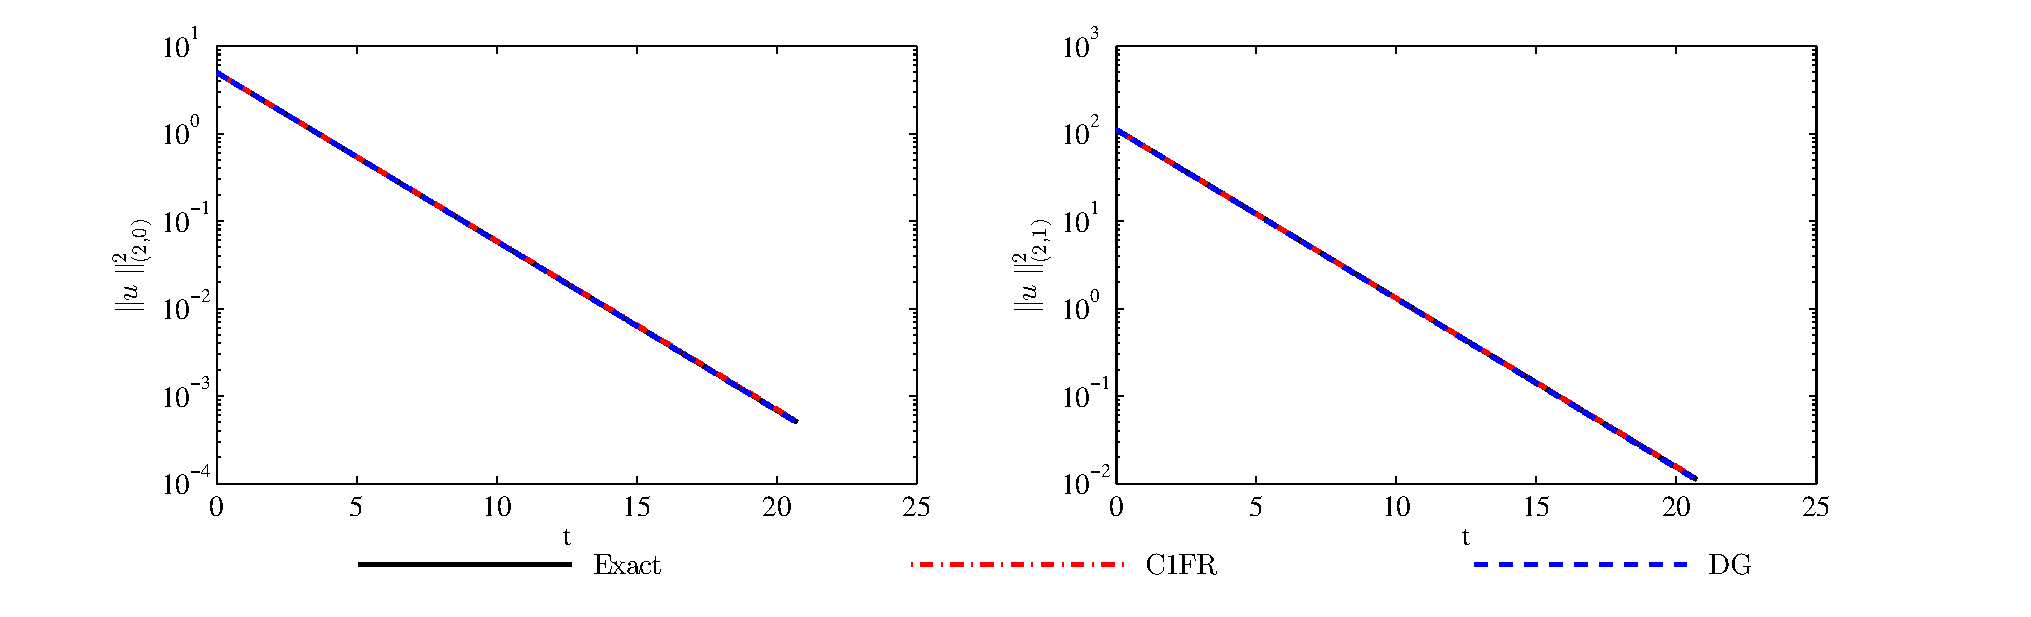
\includegraphics[width=1\textwidth,trim=\Ltrim cm 0cm \Rtrim cm 0cm]{\cmfrdir/Figures/Test_adv_diff/low_k}
\caption{Time history of norms of numerical solutions to the advection-diffusion equation and their first derivative. Initial condition is a sine wave with low wavenumber: $k = 0.25 (P+1)\pi/h$, $P = 3$, $h = 1$.}
\label{fig:low_wavenumber}
\end{figure}

\begin{figure}[h]
\centering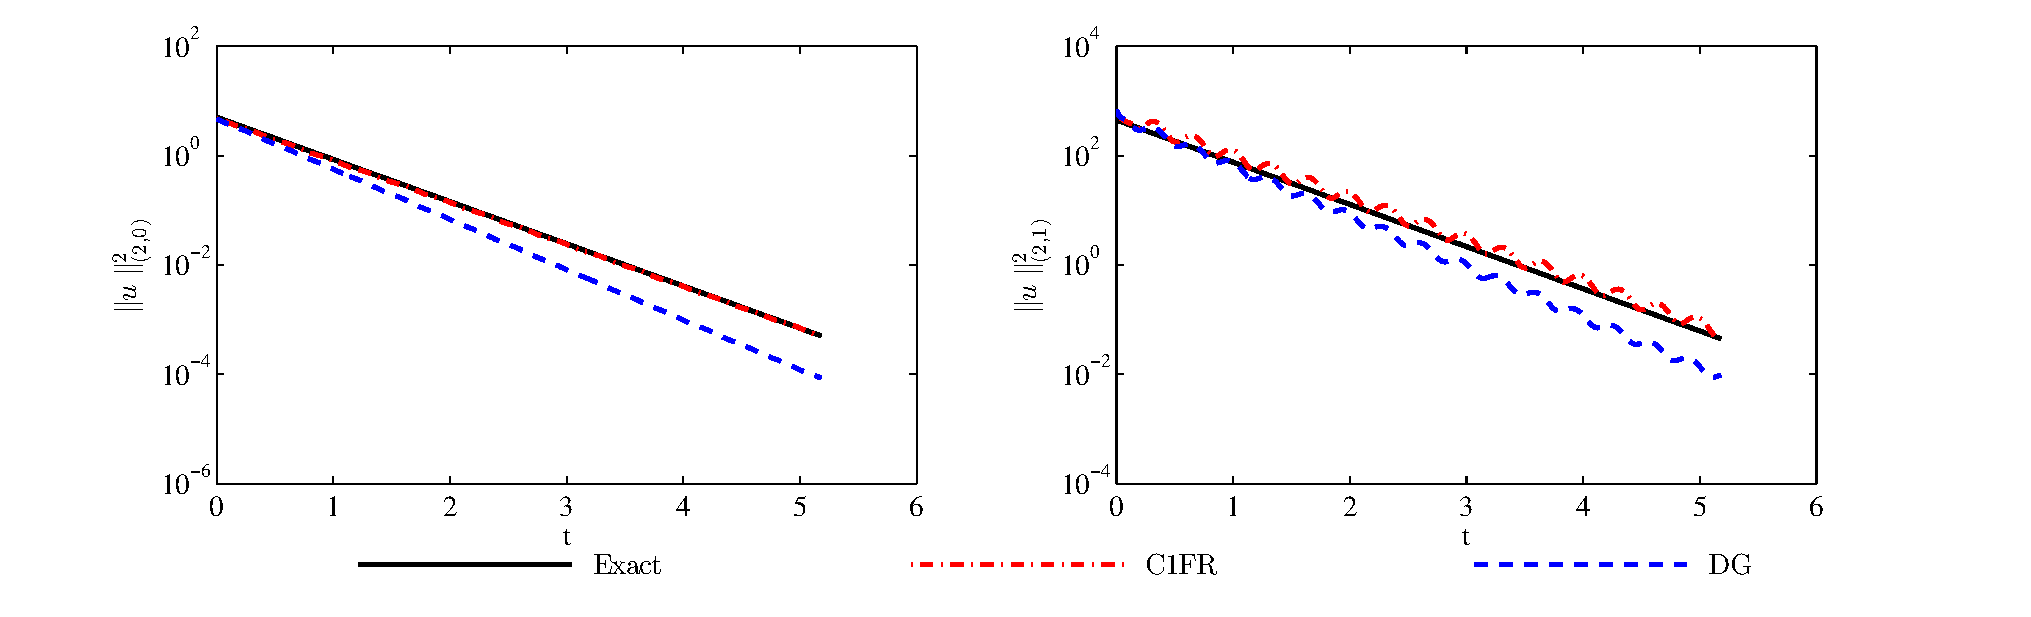
\includegraphics[width=1\textwidth,trim=\Ltrim cm 0cm \Rtrim cm 0cm]{\cmfrdir/Figures/Test_adv_diff/med_k}
\caption{Time history of norms of numerical solutions to the advection-diffusion equation and their first derivative. Initial condition is a sine wave with medium wavenumber: $k = 0.5 (P+1)\pi/h$, $P = 3$, $h = 1$.}
\label{fig:medium_wavenumber}
\end{figure}

\begin{figure}[h]
\centering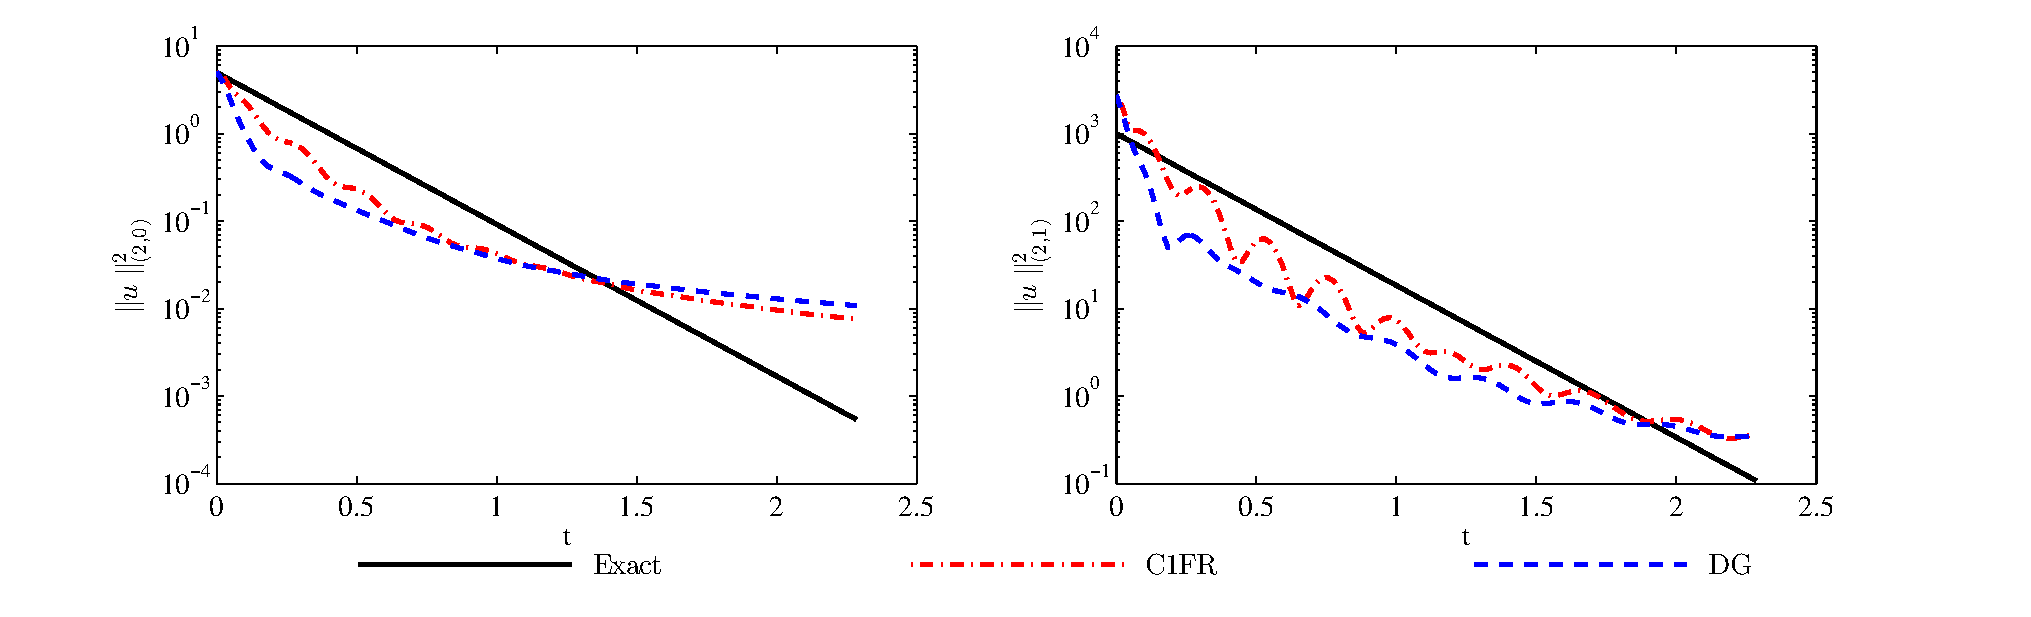
\includegraphics[width=1\textwidth,trim=\Ltrim cm 0cm \Rtrim cm 0cm]{\cmfrdir/Figures/Test_adv_diff/high_k}
\caption{Time history of norms of numerical solutions to the advection-diffusion equation and their first derivative. Initial condition is a sine wave with high wavenumber: $k = 0.75 (P+1)\pi/h$, $P = 3$, $h = 1$.}
\label{fig:high_wavenumber}
\end{figure}

%_ %_ %_ %_ %_ %_ %_ %_ %_ %_ %_ %_ %_ %_ %_ %_ %_ %
%\begin{figure}[h]
%\centering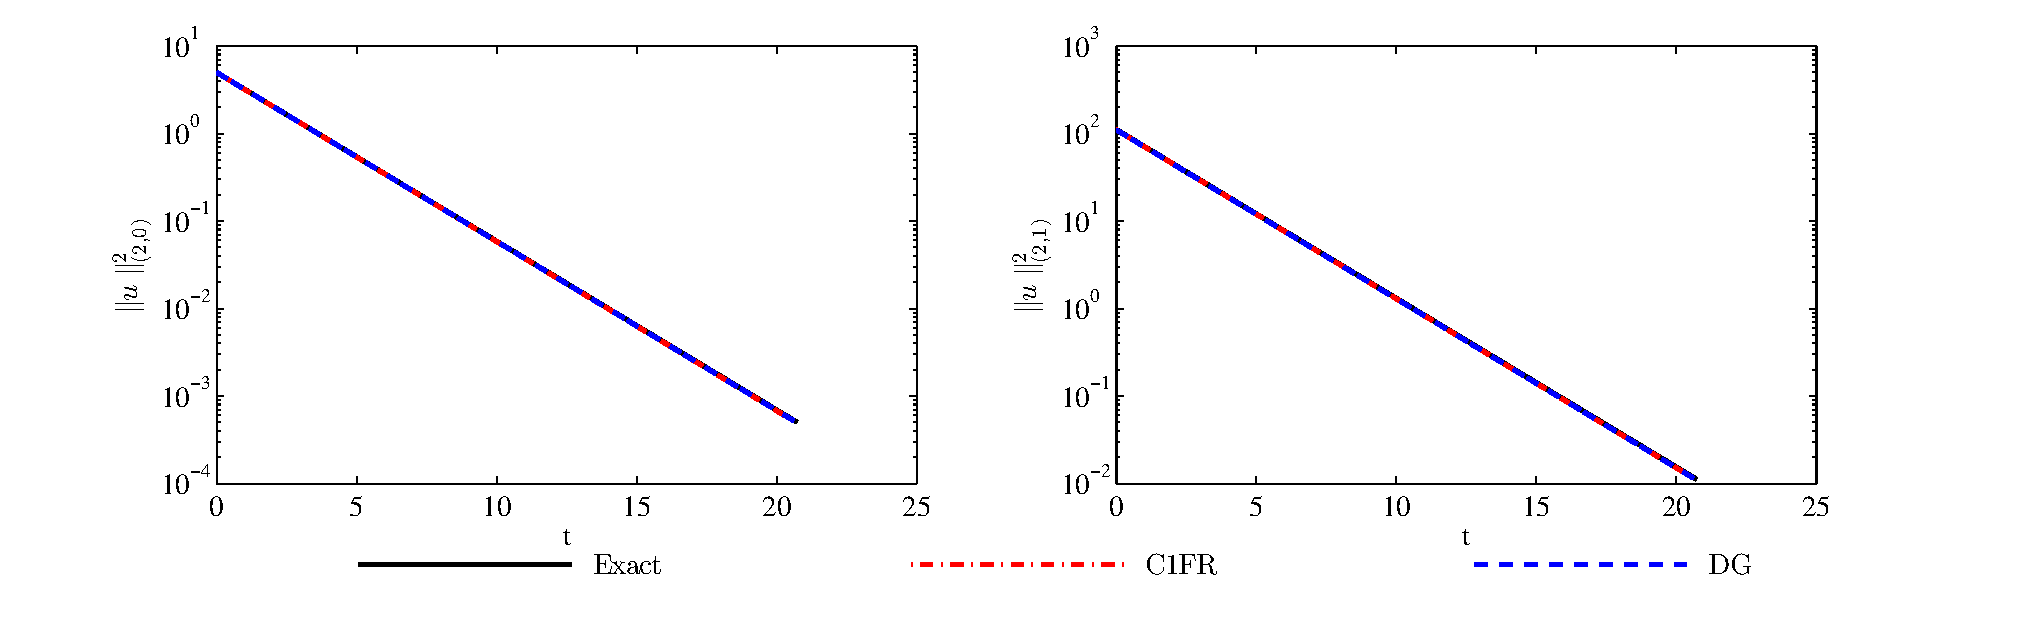
\includegraphics[width=1\textwidth,trim=\Ltrim cm 0cm \Rtrim cm 0cm]{Figures/Test_adv_diff/low_k_c_5e-3}
%\caption{Time history of norms of numerical solutions to the advection-diffusion equation and their first derivative. Initial condition is a sine wave with low wavenumber: $k = 0.25 (P+1)\pi/h$, $P = 3$, $h = 1$.}
%\label{fig:low_wavenumber2}
%\end{figure}
%
%\begin{figure}[h]
%\centering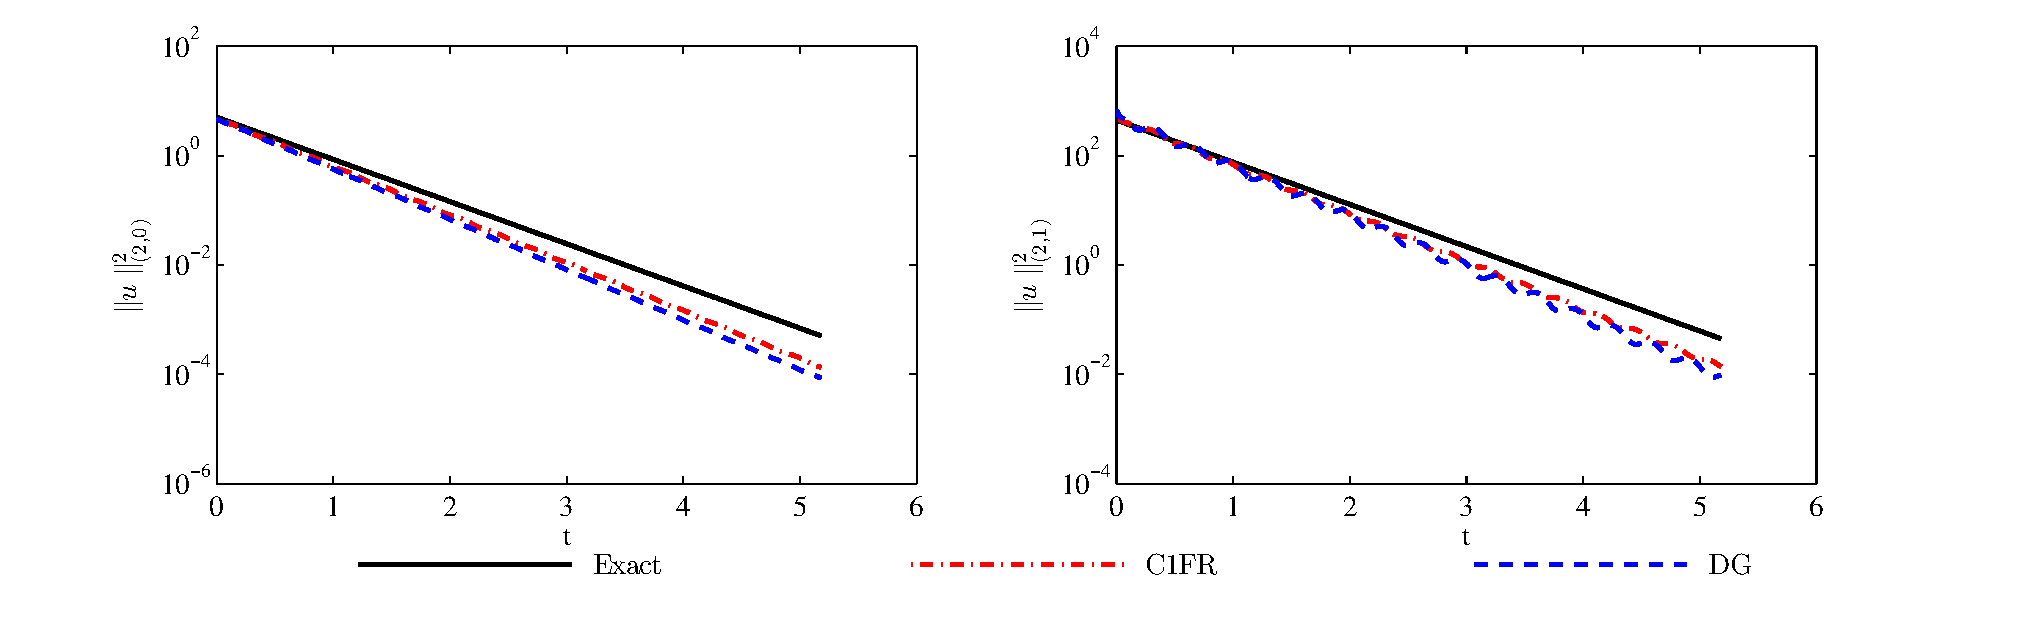
\includegraphics[width=1\textwidth,trim=\Ltrim cm 0cm \Rtrim cm 0cm]{Figures/Test_adv_diff/med_k_c_5e-3}
%\caption{Time history of norms of numerical solutions to the advection-diffusion equation and their first derivative. Initial condition is a sine wave with medium wavenumber: $k = 0.5 (P+1)\pi/h$, $P = 3$, $h = 1$.}
%\label{fig:medium_wavenumber2}
%\end{figure}
%
%\begin{figure}[h]
%\centering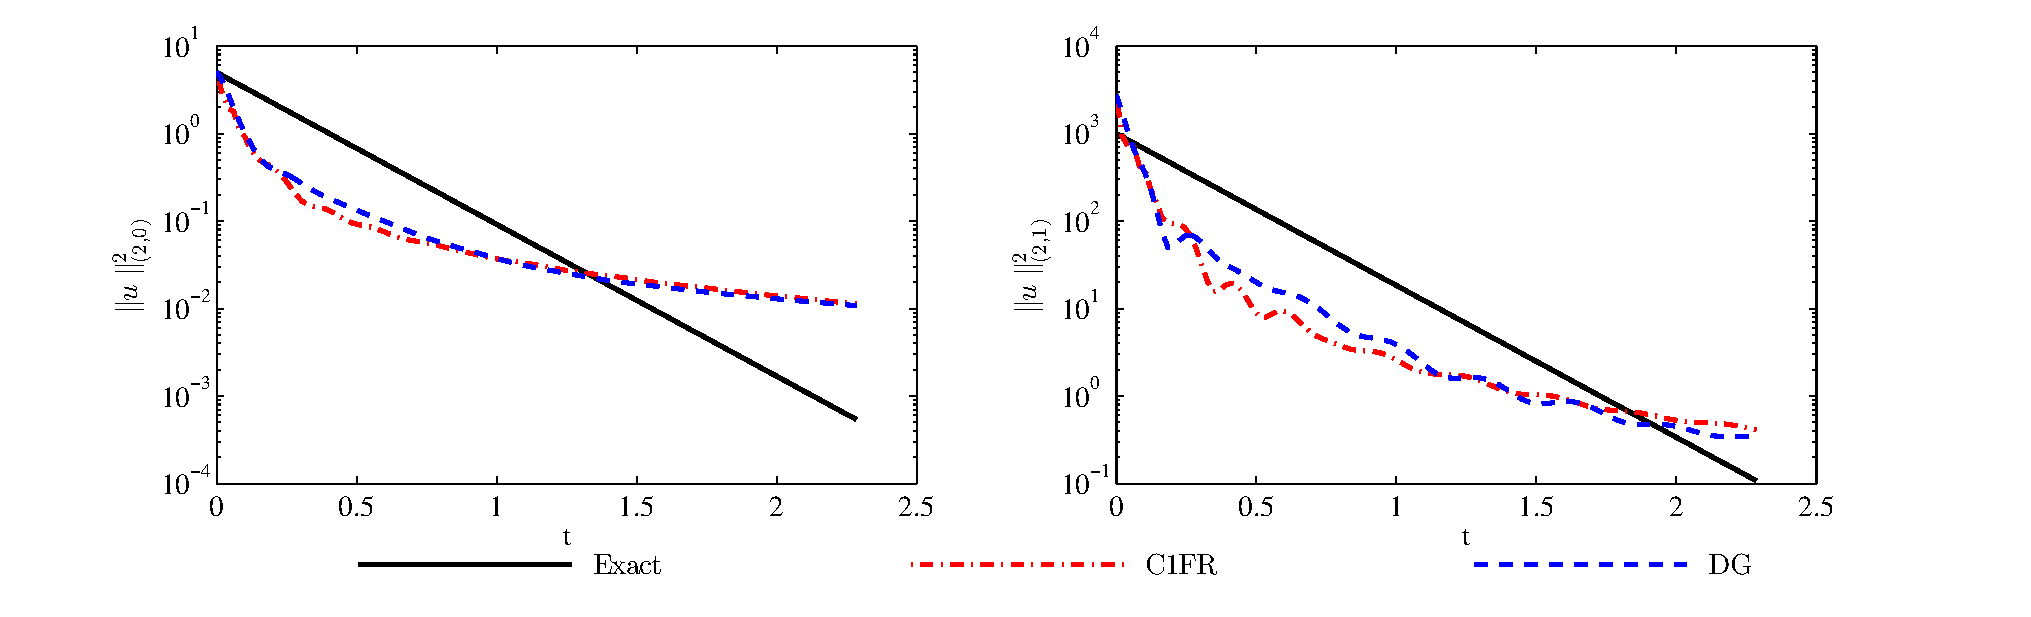
\includegraphics[width=1\textwidth,trim=\Ltrim cm 0cm \Rtrim cm 0cm]{Figures/Test_adv_diff/high_k_c_5e-3}
%\caption{Time history of norms of numerical solutions to the advection-diffusion equation and their first derivative. Initial condition is a sine wave with high wavenumber: $k = 0.75 (P+1)\pi/h$, $P = 3$, $h = 1$.}
%\label{fig:high_wavenumber2}
%\end{figure}

%_ %_ %_ %_ %_ %_ %_ %_ %_ %_ %_ %_ %_ %_ %_ %_ %_ %

%\begin{figure}
%\centering
%\subfigure[fig a]{\label{fig:high_wavenumber} 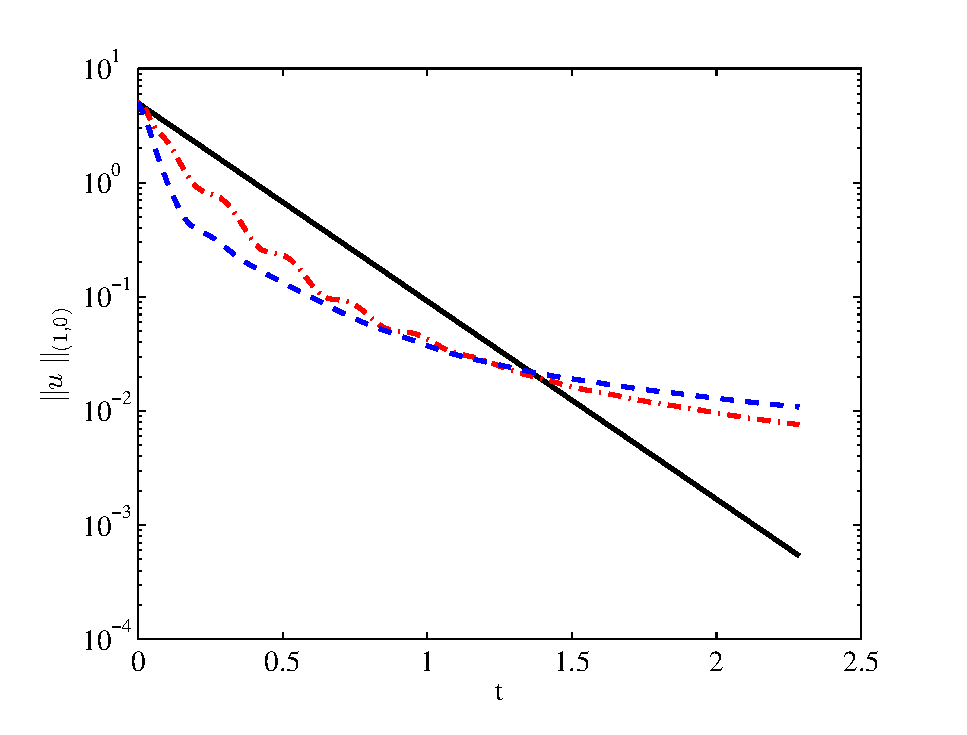
\includegraphics[width = .5\textwidth]{Figures/Test_adv_diff/eN0_high_k}
%\caption{energy history}}

%\end{subfig}
%\end{figure}



\subsection{Solutions to the Euler Equations}
\label{sec:cm1frEuler}
\subsubsection{Setup}

Solving the 1-D Euler equations is a good test of a scheme's robustness and potential for solving challenging Navier-Stokes cases. In this section we compare the performance of \gls{c1fr} to that of unmodified \gls{dg}. The equations in conservative form are

 \begin{equation}\label{1dEuler}
\frac{\partial U}{\partial t} +  \frac{\partial F}{\partial x}  = 0
\end{equation}

where 
\begin{equation}
U = \l(
\begin{tabular}{c}
$\rho$\\
$\rho u$\\
$E$
\end{tabular}
\r), 
\;\;
F = \l(
\begin{tabular}{c}
$\rho u$\\
$\rho u^2 + p$\\
$ u (E + p)$
\end{tabular}
\r), 
\end{equation}

\begin{equation}
E = \l(e + \frac{1}{2}u^2 \r) \rho,
\end{equation}
and 
\begin{equation}
p = (\gamma -1) \l(E - \frac{1}{2}\rho u^2\r).
\end{equation}

$\gamma, \rho, e$ are the usual symbols of ratio of specific heat capacities of the gas, density, and specific internal energy, respectively.

We can rewrite the system of equations so only three variables appear:
\begin{equation}
U = \l(
\begin{tabular}{c}
$U_1$\\
$U_2$\\
$U_3$
\end{tabular}
\r), 
\;\;
F = \l(
\begin{tabular}{c}
$U_2$\\
$\frac{U_2^2}{U_1} + p$\\
$\frac{U_2}{U_1} \l( U_3 + p\r)$
\end{tabular}
\r), \;\;
p = (\gamma - 1)  \l(U_3 - \frac{1}{2} \frac{U_2^2}{U_1}\r)
\end{equation}

It is possible to find exact solutions to problems with initial conditions of the form
\begin{equation*}
\rho(x,0) = \bigg\{
\begin{tabular}{c}
$
\begin{aligned}
\rho_L &\text{ if } x < x_{ref}\\
\rho_R &\text{ if } x \ge x_{ref}
\end{aligned}
$
\end{tabular},
\end{equation*}
\begin{equation}
\label{euler_initConditions}
p(x,0) = \bigg\{
\begin{tabular}{c}
$
\begin{aligned}
p_L &\text{ if } x < x_{ref}\\
p_R &\text{ if } x \ge x_{ref}
\end{aligned}
$
\end{tabular}, \text{ and }
\end{equation}
\begin{equation*}
 u(x,0) =\bigg\{
\begin{tabular}{c}
$
\begin{aligned}
u_L &\text{ if } x < x_{ref}\\
u_R &\text{ if } x \ge x_{ref}
\end{aligned}
$
\end{tabular}.
\end{equation*}
where subscripts $R,L$ mean the value is constant to the right and left, respectively, of the point $x_{ref}$. A thorough description on how to find such exact solutions is in Section 4.2 in \cite{solvers1997numerical}.

High order methods are known to not perform well in the presence of shocks. This is specially true when the initial condition is discontinuous. \gls{c1fr} schemes are not impervious to this problem and become unstable at any \gls{cfl} with discontinuous initial conditions such as those in Eqn. \eqref{euler_initConditions}.

In order to produce a solution, the initial discontinuity is ``thickened'' by using a hyperbolic tangent ($\tanh$) function, as opposed to a Heaviside step function, to step from the left value to the right value. For the following results, 
\begin{equation}
y = \frac{y_R - y_L}{2} \tanh(K (x - x_{ref})) + \frac{y_R + y_L}{2}
\end{equation}

where $y$ is the quantity being initialized ($\rho, p, u$) and $K$ modifies the sharpness of the step. When $K \rightarrow \infty$, we recover the Heaviside step function. A value of $K=90$ produced a subjectively appropriate sharpness and allowed the numerical solution to develop shocks by itself. We are interested in seeing how the numerical scheme handles the latter.

Even though the initial conditions were modified, it is still possible to observe that the \gls{c1fr} functions have enhanced built-in resilience relative to regular \gls{dg}.

No modifications to the interface flux definitions were made for the following results.  It can be argued that a different selection of fluxes and the use of limiters or filters could improve the results of both \gls{c1fr} and \gls{dg}. However, the goal of the following exposition is not to present the ``best'' or a ``better'' numerical scheme for the solution of the Euler equations, but rather to assess the behavior of a general scheme like \gls{c1fr} in a challenging situation that could appear in a flow of engineering interest. The idea behind this goal is that if an untuned scheme performs well in a challenging scenario, it is reasonable to expect the engineer will not need to spend much time and effort tuning the simulation parameters to obtain a useful solution to a problem.

\subsubsection{Results and discussion}
\setcounter{secnumdepth}{5}
\paragraph{Sod's Shock Tube}
\label{sec:shock_tube}
The initial conditions for this problem are, as shown in \cite{roe1981approximate},
\begin{equation*}
\rho(x,0) = \bigg\{
\begin{tabular}{c}
$
\begin{aligned}
1 &\text{ if } x < 0.5\\
0.123 &\text{ if } x \ge 0.5
\end{aligned}
$
\end{tabular},\;\;
p(x,0) = \bigg\{
\begin{tabular}{c}
$
\begin{aligned}
1 &\text{ if } x < 0.5\\
0.1 &\text{ if } x \ge 0.5
\end{aligned}
$
\end{tabular}
,\text{ and } u(x,0) = 0.
\end{equation*}

Figure \ref{c1fr_shockTube_initCond} plots the initial conditions with the ``thickened'' discontinuity.

\begin{figure}
\centering
\hspace{-1.25 cm}
\centering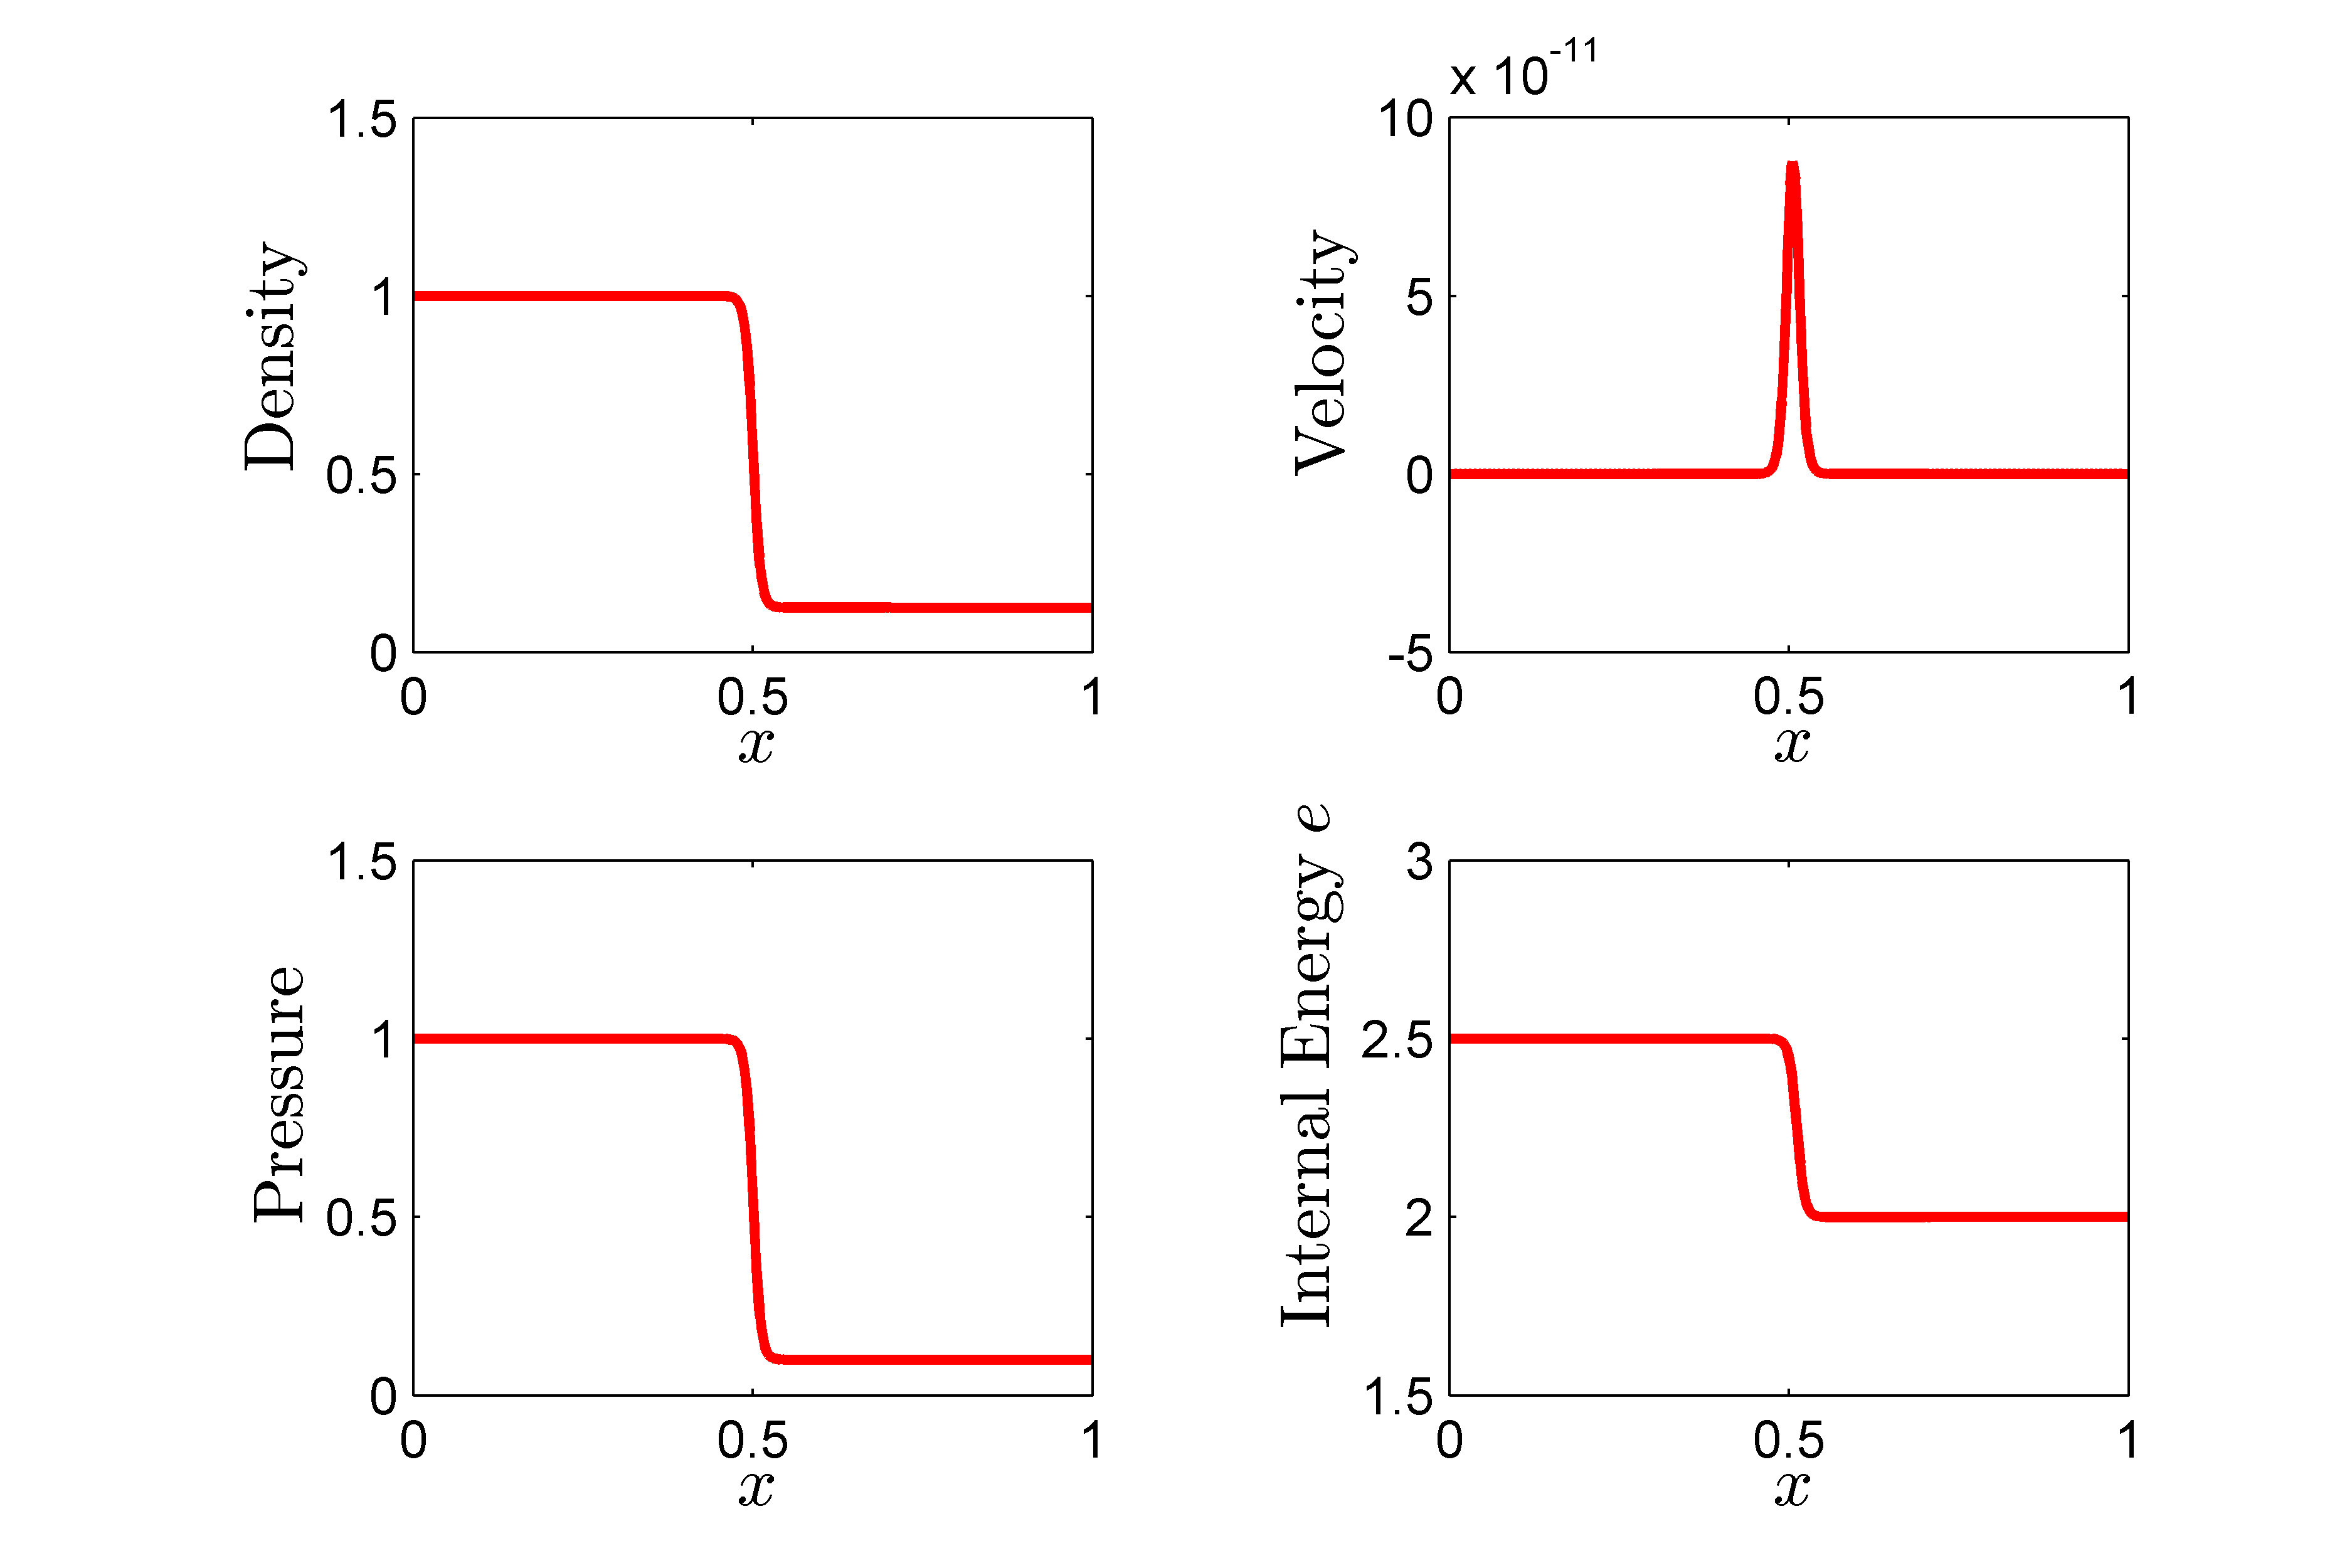
\includegraphics[width=0.525\textwidth,trim=\Ltrim cm 0cm \Rtrim cm 0cm]{\cmfrdir/Figures/Euler/Euler_shockTube_initCond.png}
  \caption{Sod's Shock Tube Problem with ``thickened'' discontinuity at $t = 0$.}
  \label{c1fr_shockTube_initCond}
\end{figure}

Figure \ref{c1fr_shockTube} shows the results to this problem at $t=0.25$ s using \gls{c1fr}. The flux used in the $0^{\mathrm{th}}$ derivative is central ($\alpha_0 = 1$ in Eqn. \eqref{eq:ifluxdef}) and the flux used in the $1^{\mathrm{st}}$ derivative is upwinded ($\alpha_1 = 0$ in Eqn. \eqref{eq:ifluxdef}). The correction functions are created with $c_1 = 1e-2$ in Eqn. \eqref{eqn:system}. The time-stepping method was \gls{rk}4, and the \gls{cfl} for the \gls{c1fr} and \gls{dg} cases was $2.5e-2$. The timestep was set to

\begin{equation}
\label{eq:cfl_cond}
\Delta t = \frac{\mathrm{\gls{cfl}} h}{|a|+|u|}
\end{equation}
where $h$ is the element size and $|a| = \sqrt{\gamma  \frac{p}{\rho}}$ is the speed of sound.

\begin{figure}
\centering
\hspace{-1.25 cm}
\centering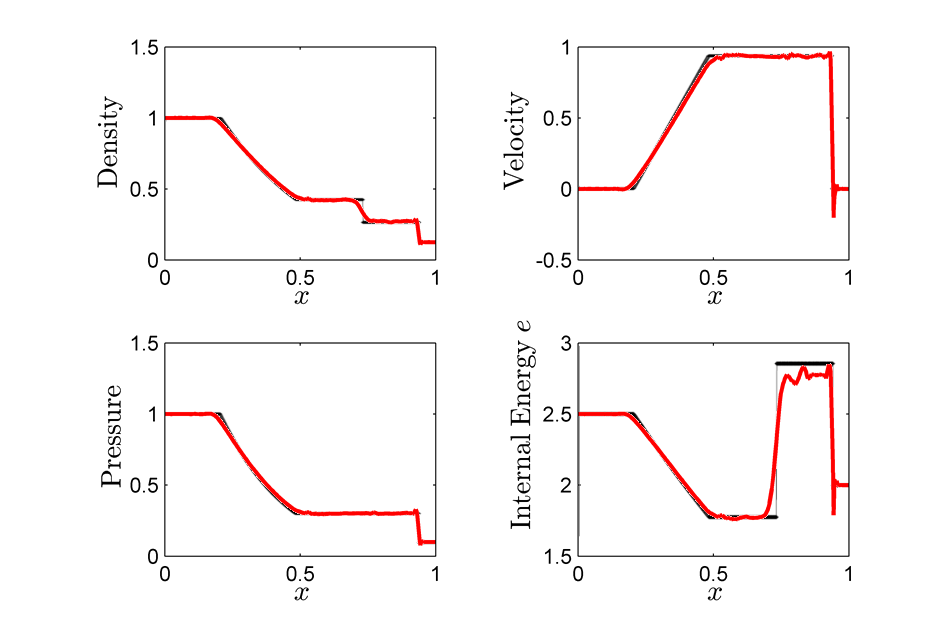
\includegraphics[width=0.2\textwidth,trim=\Ltrim cm 0cm \Rtrim cm 0cm]{\cmfrdir/Figures/Euler/Euler_shockTube.png}
  \caption{Sod's Shock Tube Problem at $t = 0.25$ solved with \gls{c1fr}. Solid black line is the exact solution to the original problem with discontinuous initial conditions. Superimposed solid red line is the solution obtained with the \gls{c1fr} scheme and ``thickened'' discontinuity in the initial conditions shown in Figure \ref{c1fr_shockTube_initCond}. $N=71, P=3,  c_1 = 1e-2, \alpha_0=1, \alpha_1 = 0, \mathrm{\gls{cfl}}=2.5e-2$}
  \label{c1fr_shockTube}
\end{figure}

The solution to the Shock Tube problem with \gls{c1fr} exhibits oscillations at the contact discontinuities, as expected. During the run of this simulation, the magnitude of these oscillation increased and decreased. The maximum value of the internal energy was not achieved. It is worth noting that slight oscillations are also present at the plateaus. This is an unexpected result, as a central flux causes large oscillations beyond the discontinuity points. It could be surmised that the upwinding of the first derivative flux acted as a limiter.

Figure \ref{c1fr_shockTube_regDG} shows the solution with regular, unfiltered, non-limited \gls{dg} with the upwinded Rusanov flux ($\alpha_0 = 0$ in Eqn. \eqref{eq:ifluxdef}).

\begin{figure}
\centering
\hspace{-1.25 cm}
\centering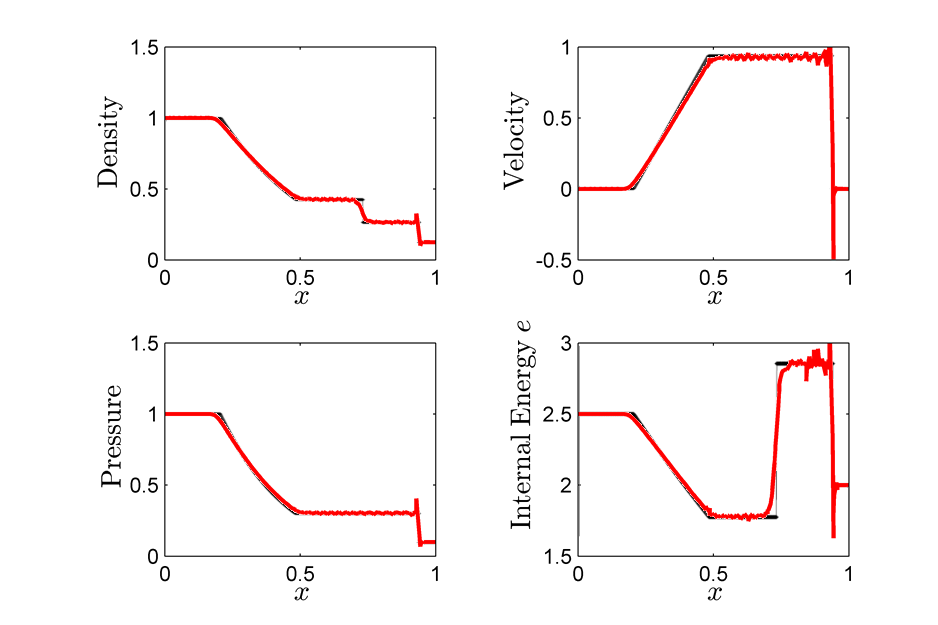
\includegraphics[width=0.2\textwidth,trim=\Ltrim cm 0cm \Rtrim cm 0cm]{\cmfrdir/Figures/Euler/Euler_shockTube_regDG.png}
  \caption{Sod's Shock Tube Problem at $t = 0.25$ solved with regular \gls{dg}. Solid black line is the exact solution to the original problem with discontinuous initial conditions. Superimposed solid red line is the solution obtained with the \gls{dg} scheme and ``thickened'' discontinuity in the initial conditions shown in Figure \ref{c1fr_shockTube_initCond}. $N=70, P=3, \alpha_0=0$}
  \label{c1fr_shockTube_regDG}
\end{figure}

The solution to the Shock Tube problem with \gls{dg} exhibits larger oscillations at the contact discontinuities than with \gls{c1fr}. The maximum value of the internal energy was achieved, albeit with very large oscillations at the discontinuity. Results by Lv et al. \cite{lv2015entropy} show that even some bounding strategies produce similar overshoot magnitudes at the discontinuities. Visible oscillations are also present at the plateaus, contrary to the results with \gls{c1fr}. This behavior is expected; \gls{dg} has been used to solve the 1-D Euler equations neatly in the presence of shocks when combined with limiters \cite{wang2015arbitrary} or filters \cite{asthana2014}. It could be surmised that the upwinding of the first derivative flux acted as a limiter.

\paragraph{123 Problem}
The 123 Problem was designed to reach conditions in which the Euler equations cannot be linearized and, hence, the Roe Flux does not provide a physical answer. It is important to note that this case is challenging for even low-order methods created specifically for the Euler equations, as seen in \cite{hudson2006review}, where the \gls{hlle} scheme \cite{einfeldt1988godunov} and \gls{ausm} \cite{liou1996sequel} are compared.
The initial conditions are, as shown in \cite{einfeldt1991godunov},
\begin{equation*}
\rho(x,0) = 1,\;\;
p(x,0) = 0.4
,\text{ and } u(x,0) = \bigg\{
\begin{tabular}{c}
$
\begin{aligned}
-2 &\text{ if } x < 0.5\\
2 &\text{ if } x \ge 0.5
\end{aligned}
$
\end{tabular}.
\end{equation*}

Figure \ref{c1fr_123_initCond} plots the initial conditions with the ``thickened'' discontinuity.

\begin{figure}
\centering
\hspace{-1.25 cm}
\centering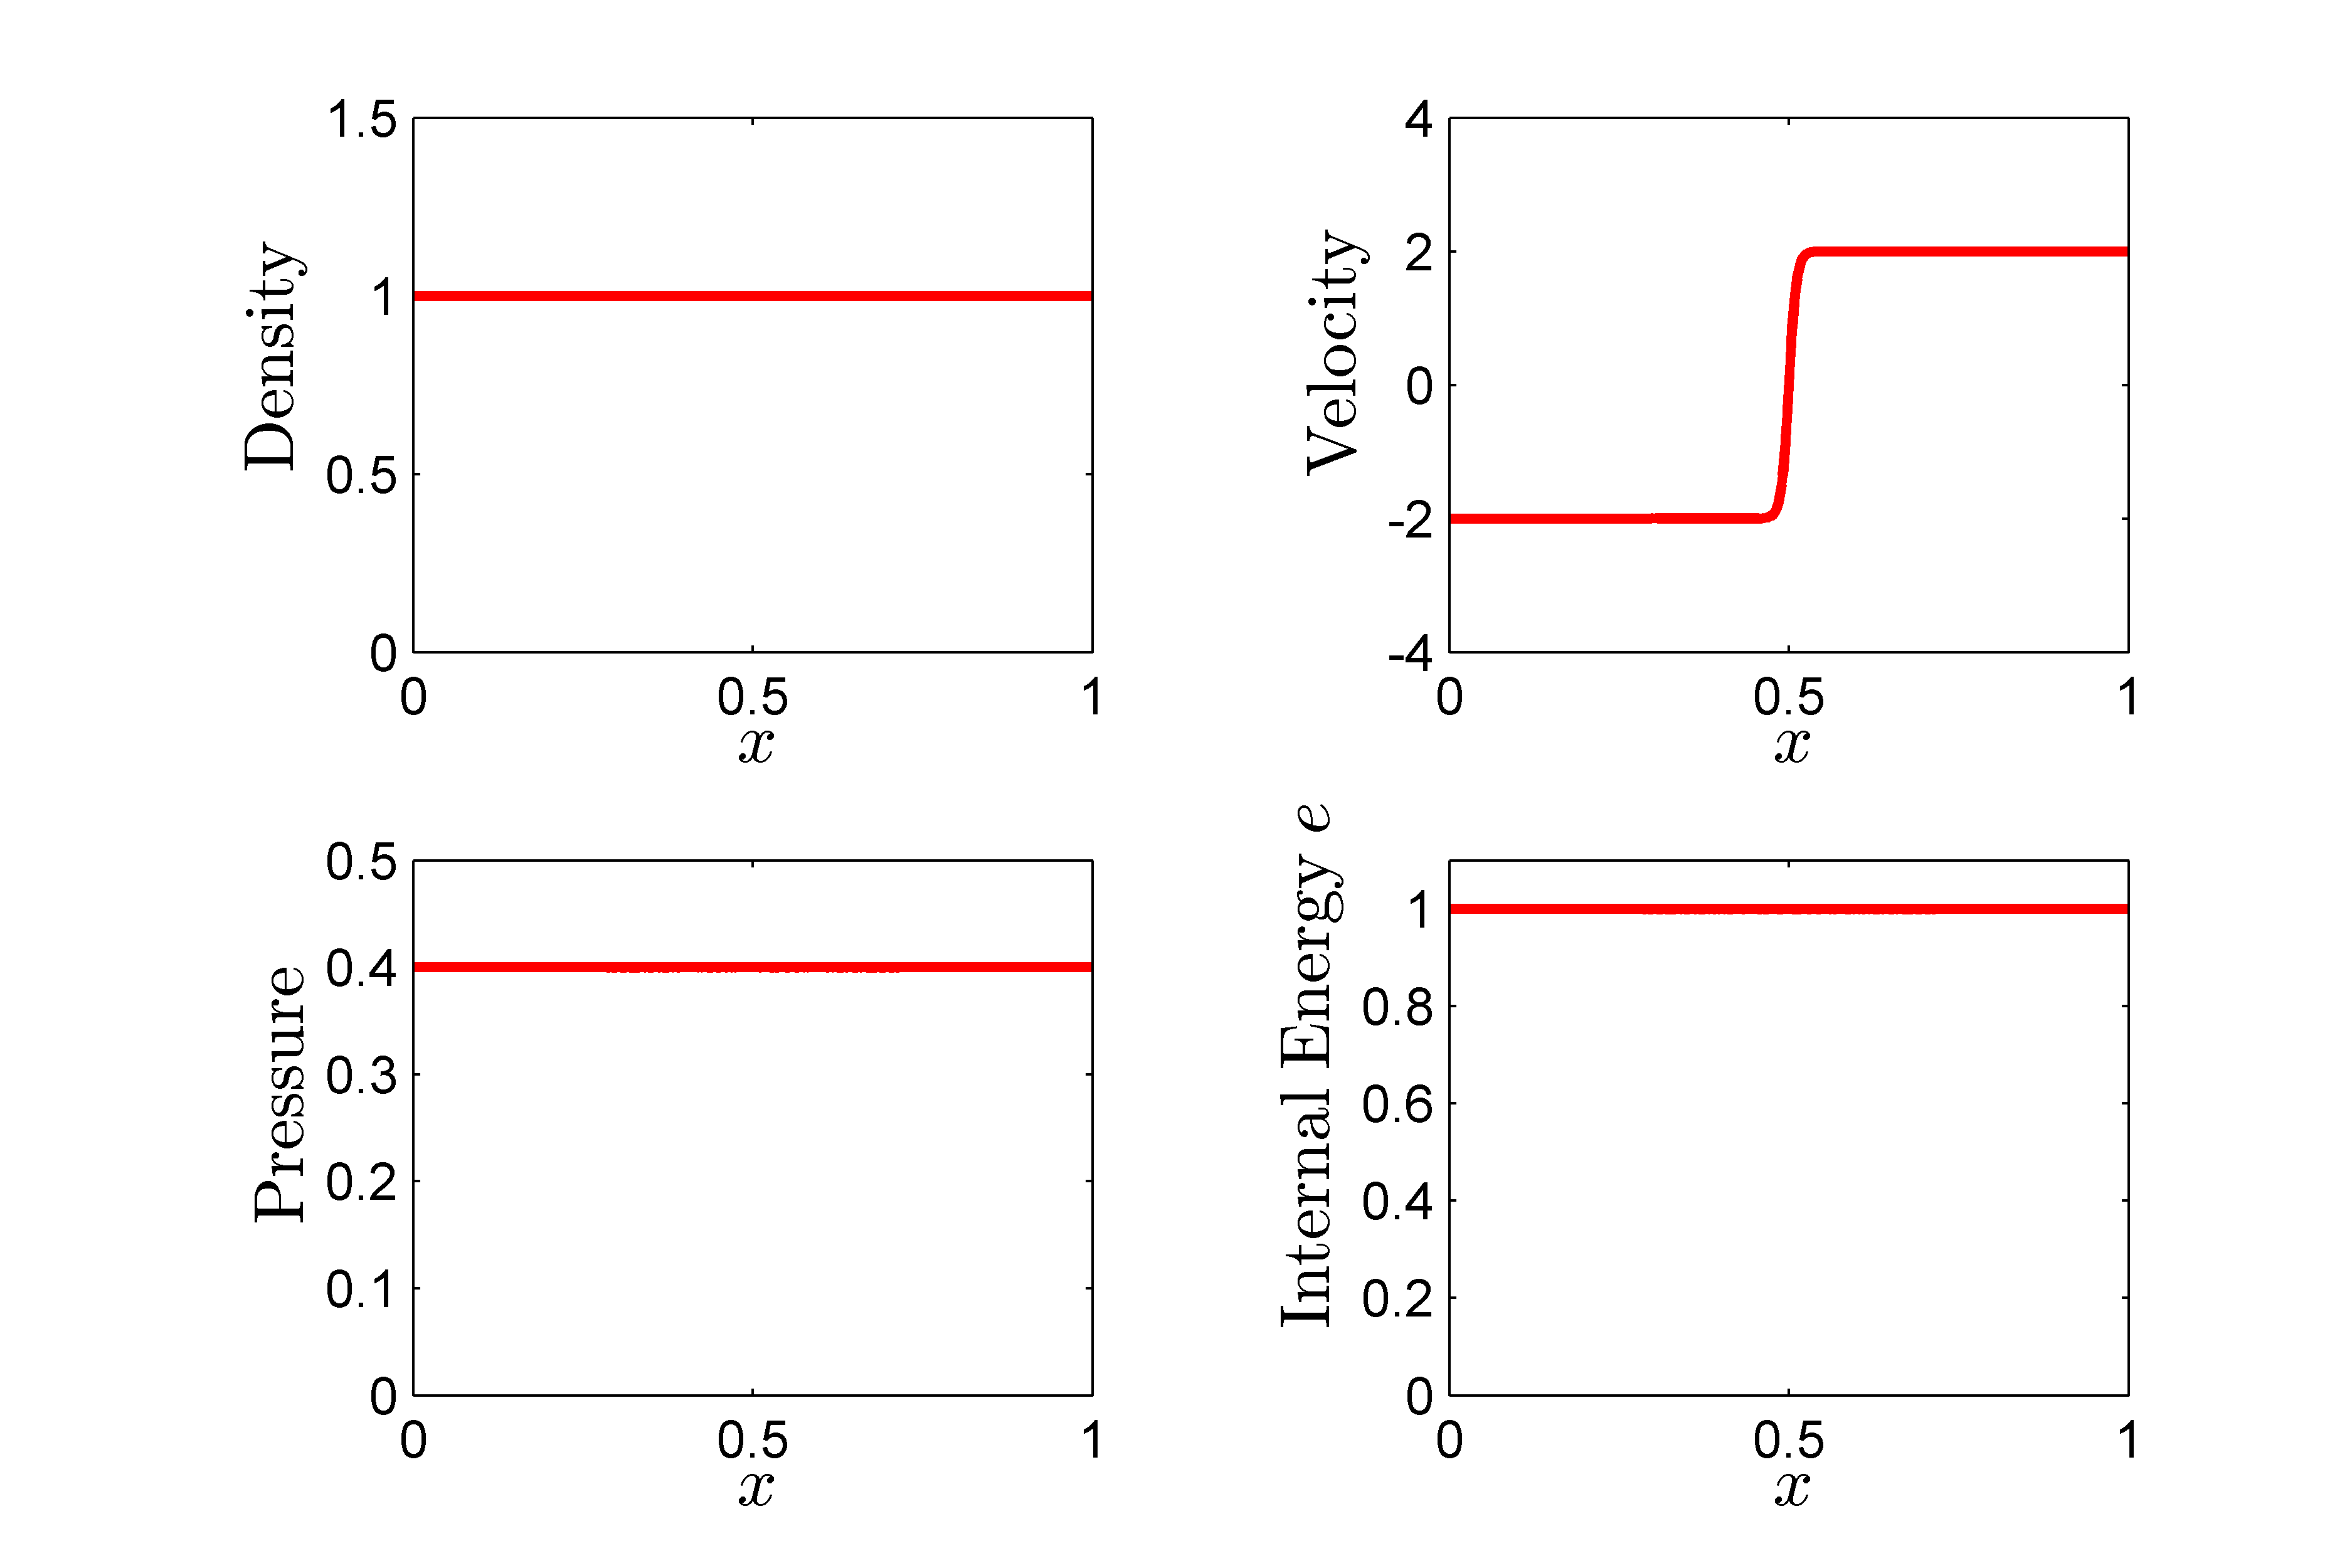
\includegraphics[width=0.525\textwidth,trim=\Ltrim cm 0cm \Rtrim cm 0cm]{\cmfrdir/Figures/Euler/Euler_123_initCond.png}
  \caption{123 Problem with ``thickened'' discontinuity at $t = 0$ solved with \gls{c1fr}. Solid black line is the exact solution to the original problem with discontinuous initial conditions. Superimposed solid red line is the solution obtained with the \gls{c1fr} scheme and ``thickened'' discontinuity in the initial conditions shown in Figure \ref{c1fr_123_initCond}. $N=71, P=3,  c_1 = 1e-2, \alpha_0=1, \alpha_1 = 0, \mathrm{\gls{cfl}}=2.5e-2$}
  \label{c1fr_123_initCond}
\end{figure}

Figure \ref{c1fr_123} shows the results at $t=0.1$ s using \gls{c1fr}. The parameters for \gls{c1fr} in this case are the same as in Section \ref{sec:shock_tube}, including the \gls{cfl}. 



Stable results with unmodified \gls{dg} could not be obtained. The reader is directed to Figure 3.4 in \cite{wang2015arbitrary} and Figure 4.3 in \cite{hudson2006review} to appreciate that accurate solutions to this problem are particularly difficult. \cite{wang2015arbitrary} needed to design fluxes for \gls{dg} to obtain a reasonable result.

The most common challenge for the schemes in the aforementioned references is that the internal energy at $x=0$ is always over-estimated. For example, as shown in \cite{hudson2006review}, \gls{hlle} overestimates $e(x=0,t=0.1)$ by $~0.1$; \gls{ausm} by $~0.8$; and \cite{wang2015arbitrary} by at least $~0.2$, even though Wang's simulations used \gls{dg} with $P=1$ (second order accurate in space). 

Given how challenging this problem is, \gls{c1fr} performed exceedingly well without the use of limiters or filters. $e(x=0,t=0.1)$ is overestimated by $~0.1$ and shows some oscillations around $x=0$. The plateau in $u(x=0, t=0.1)$ is missed (likely because of the ``thickened'' discontinuous initial conditions). This type of result suggests that \gls{c1fr} could be robust enough for flows of engineering interest.
\begin{figure}
\centering
\hspace{-1.25 cm}
\centering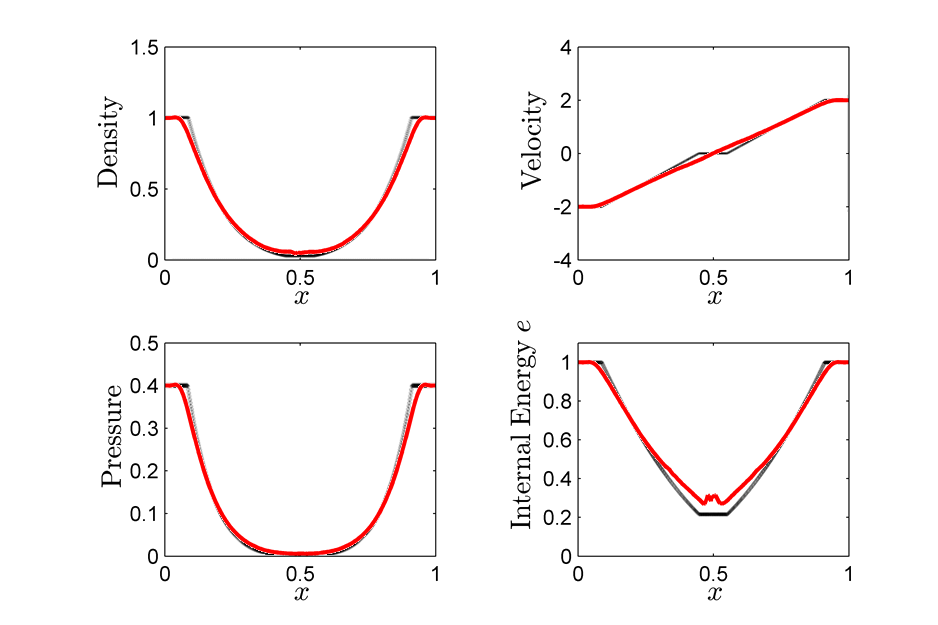
\includegraphics[width=0.2\textwidth,trim=\Ltrim cm 0cm \Rtrim cm 0cm]{\cmfrdir/Figures/Euler/Euler_123.png}
  \caption{123 problem at $t = 0.1$. Solid black line is the exact solution. Superimposed solid red line is the solution obtained with the \gls{c1fr} scheme.}
  \label{c1fr_123}
\end{figure}